\clearpage
%\newpage

\setcounter{figure}{0}
\renewcommand\thefigure{A.\arabic{figure}}    

\setcounter{table}{0}
\renewcommand{\thetable}{A.\arabic{table}}
\setcounter{subsection}{0}

\begin{center}
\huge
\textbf{Appendix: NOT FOR PUBLICATION}
\normalsize
\end{center}


\section*{Appendix A: Additional Tables and Figures} \label{sec:appa}
\newpage



\begin{figure}[htbp]
         \centering
        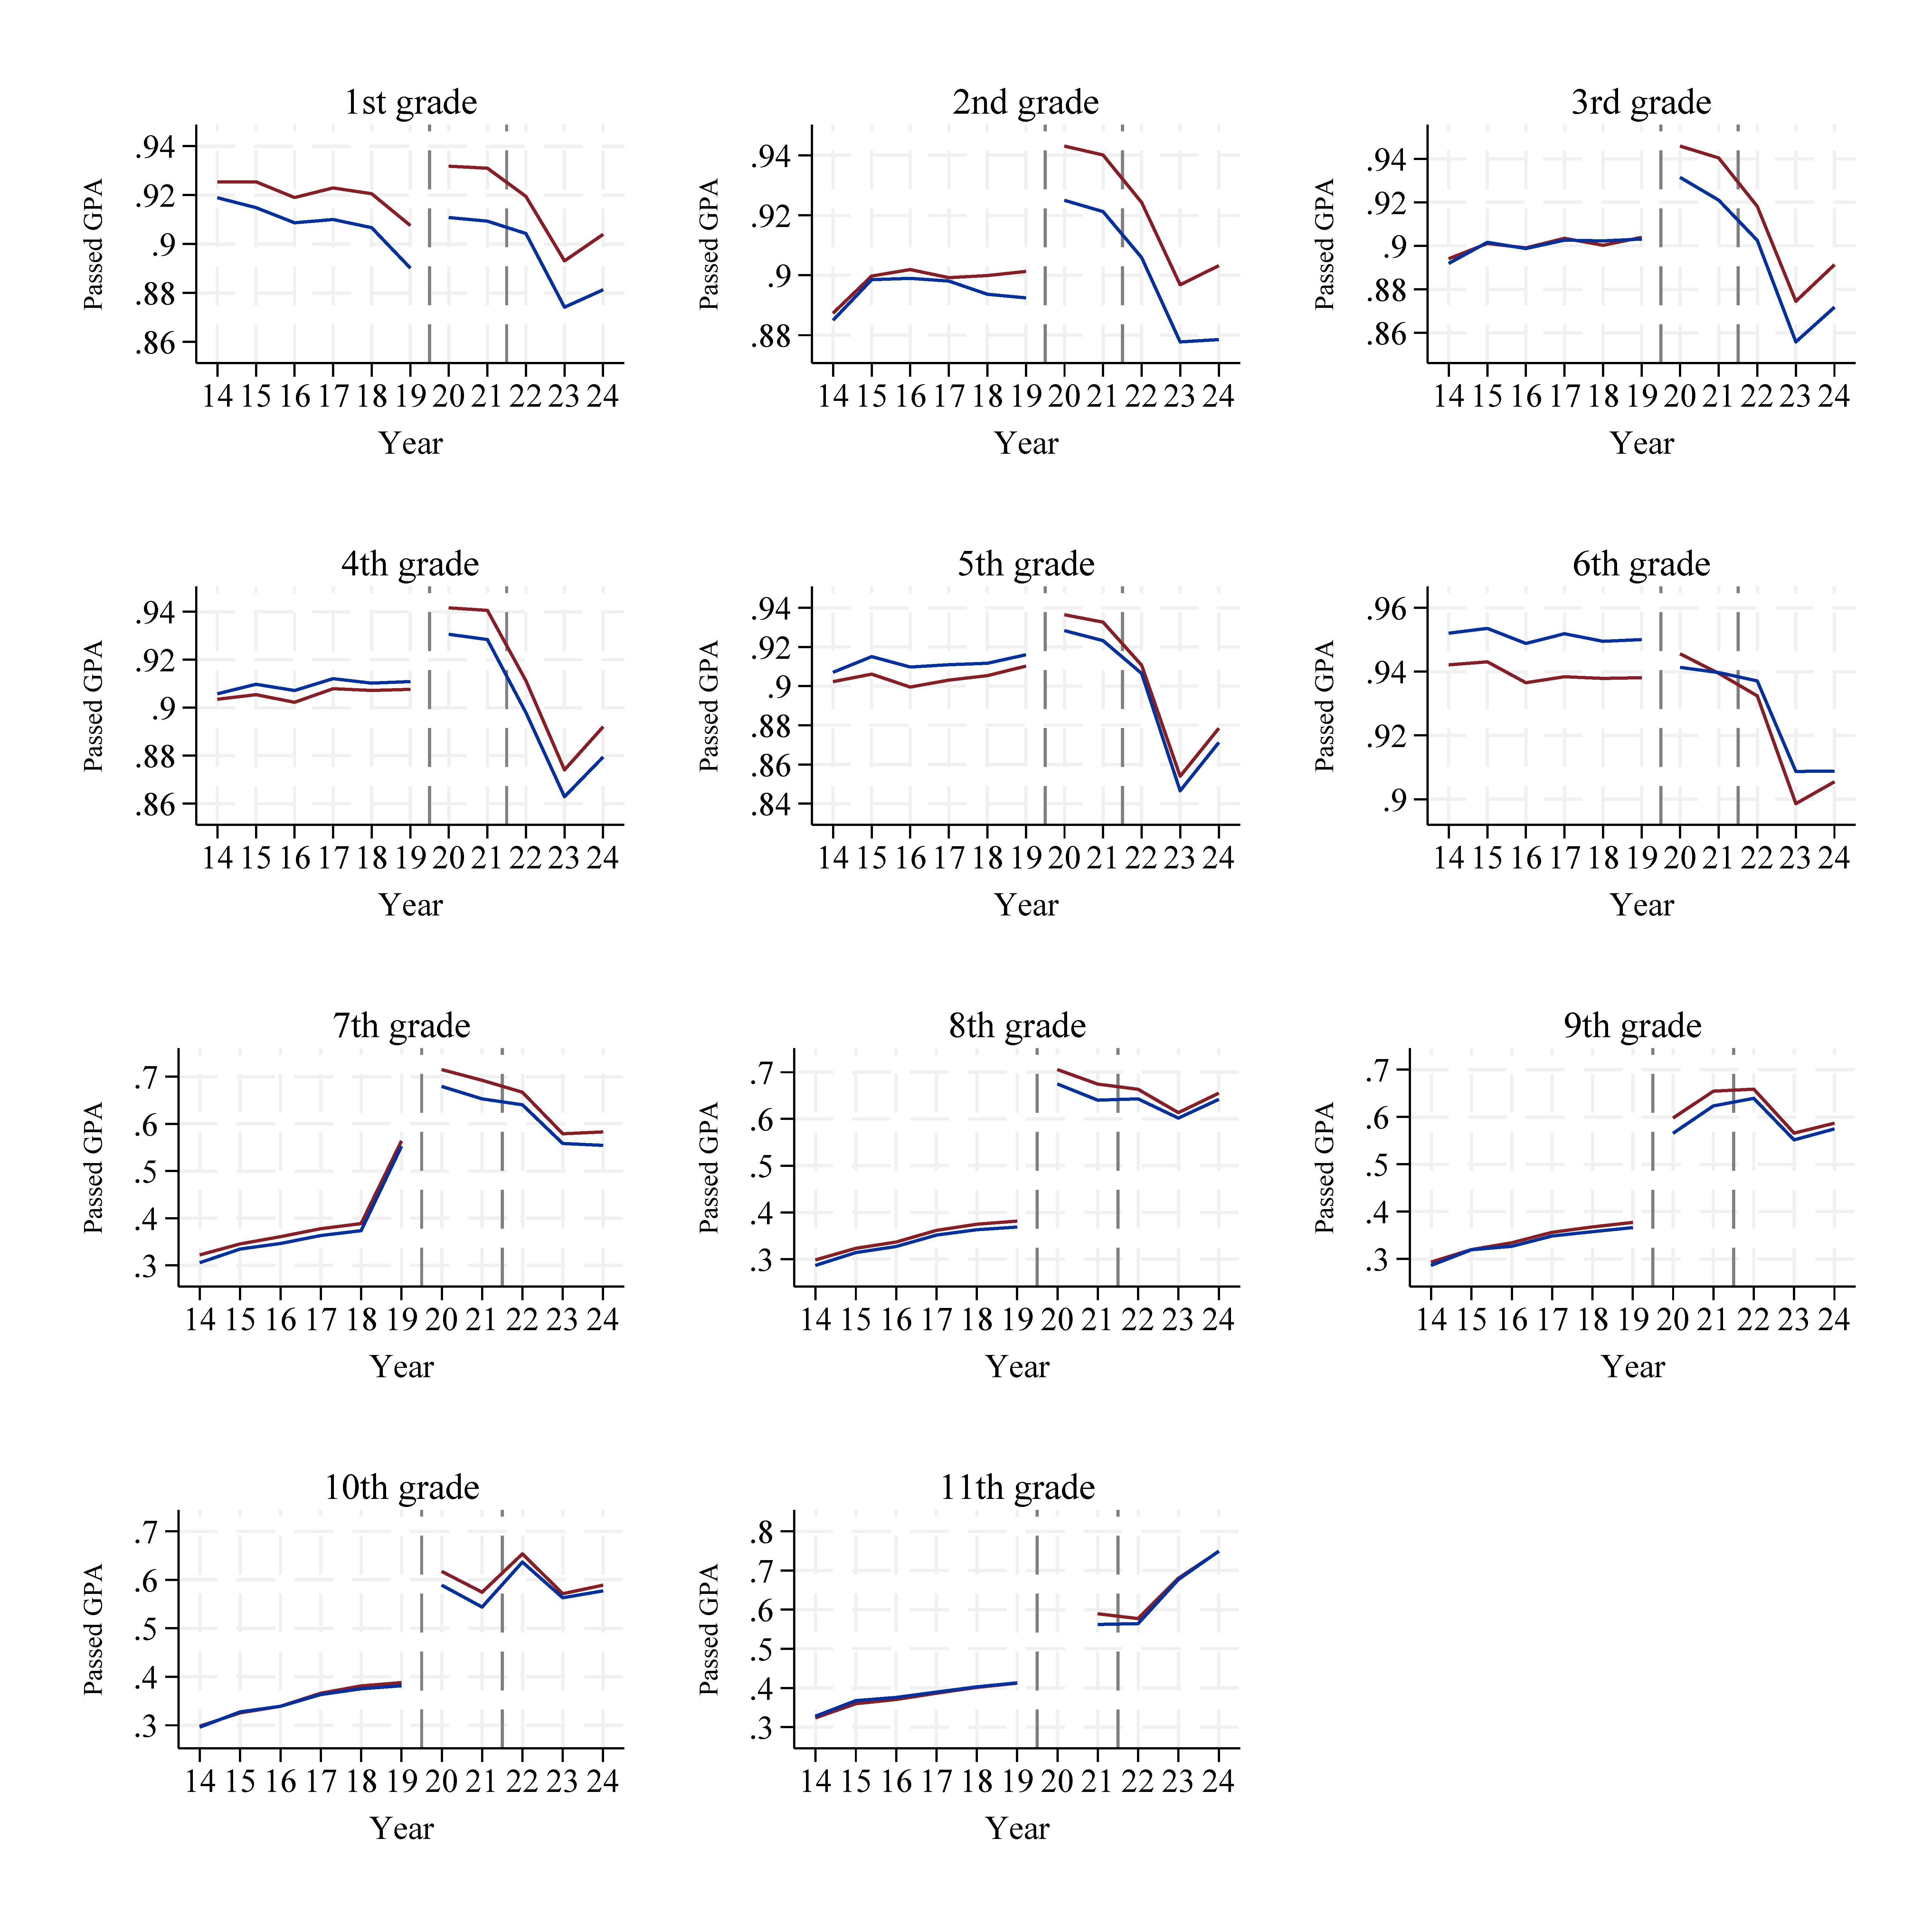
\includegraphics[width=\textwidth]{./FIGURES/Descriptive/raw_grades_pass_math_siblings.pdf}
        \caption{\% of students with an A in Mathematics for each grade 1st-1th}
        \label{fig:trend_pass_grades}
\end{figure}

\begin{figure}[htbp]
         \centering
        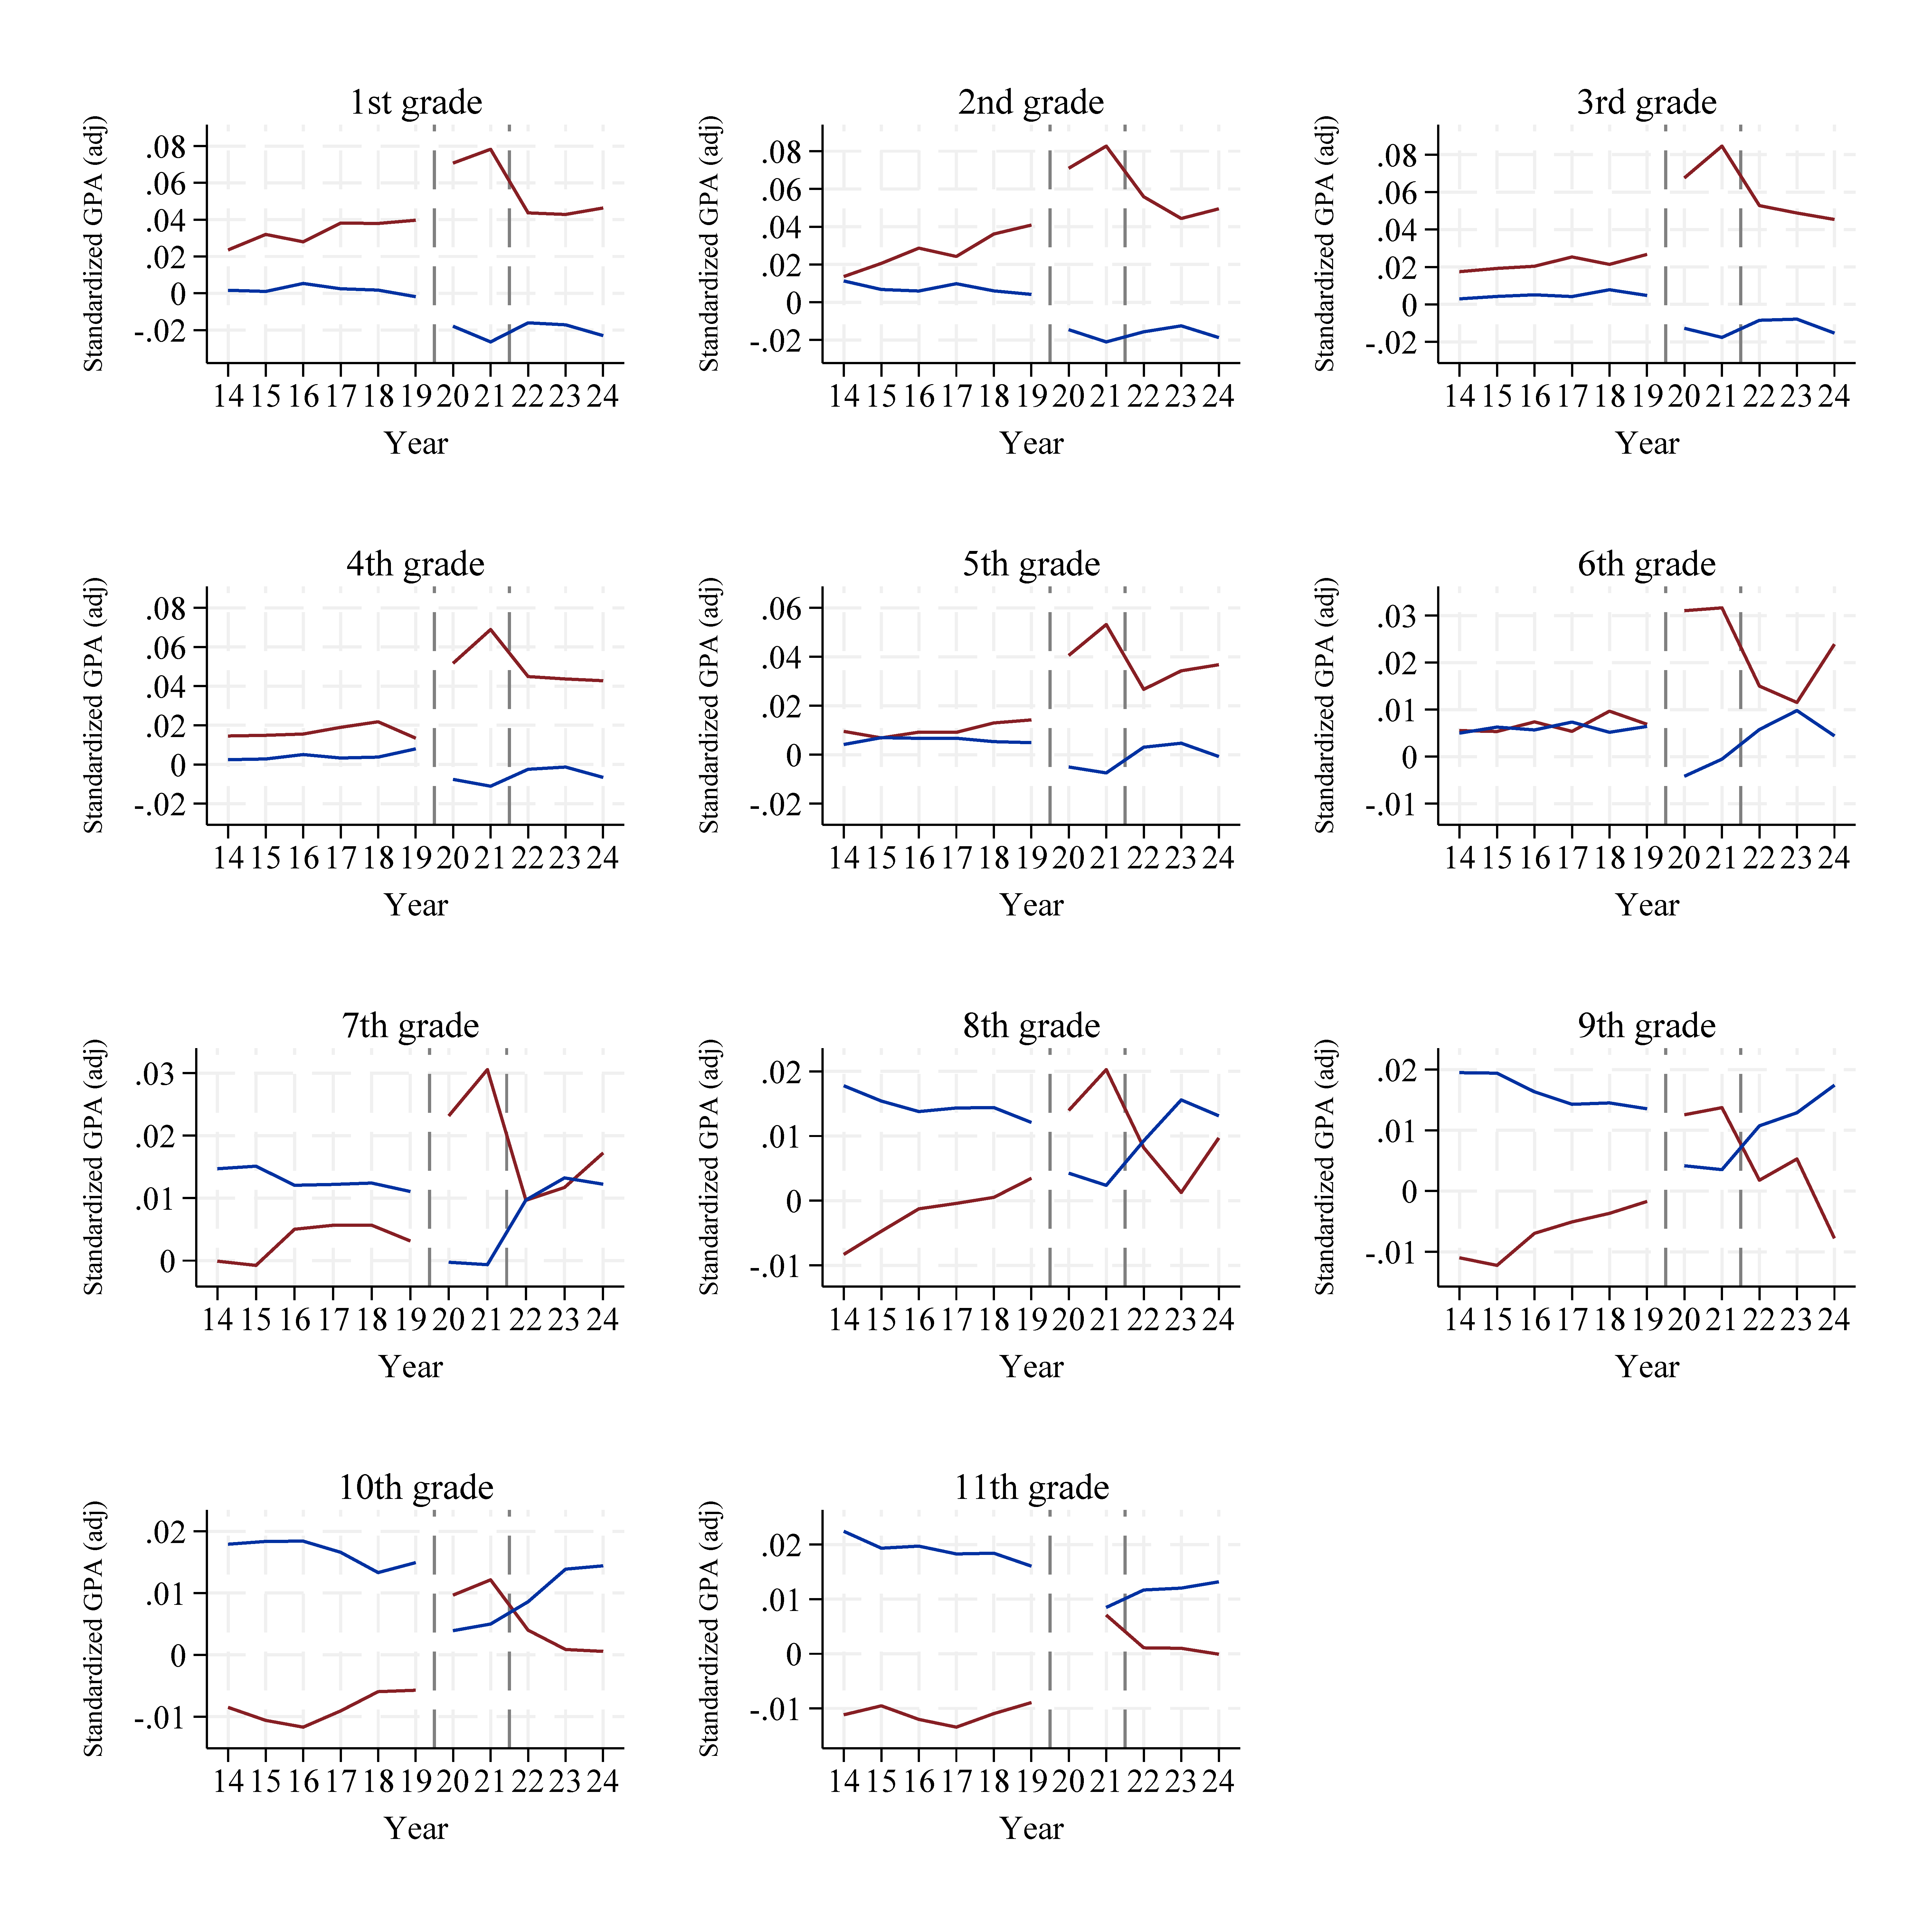
\includegraphics[width=\textwidth]{./FIGURES/Descriptive/raw_grades_std_gpa_m_adj_siblings.pdf}
        \caption{Average GPA standardized within school-grade-year for each grade 1st-1th}
        \label{fig:trend_gpa_grades}
\end{figure}



\begin{figure}[htbp]
    \centering
    
        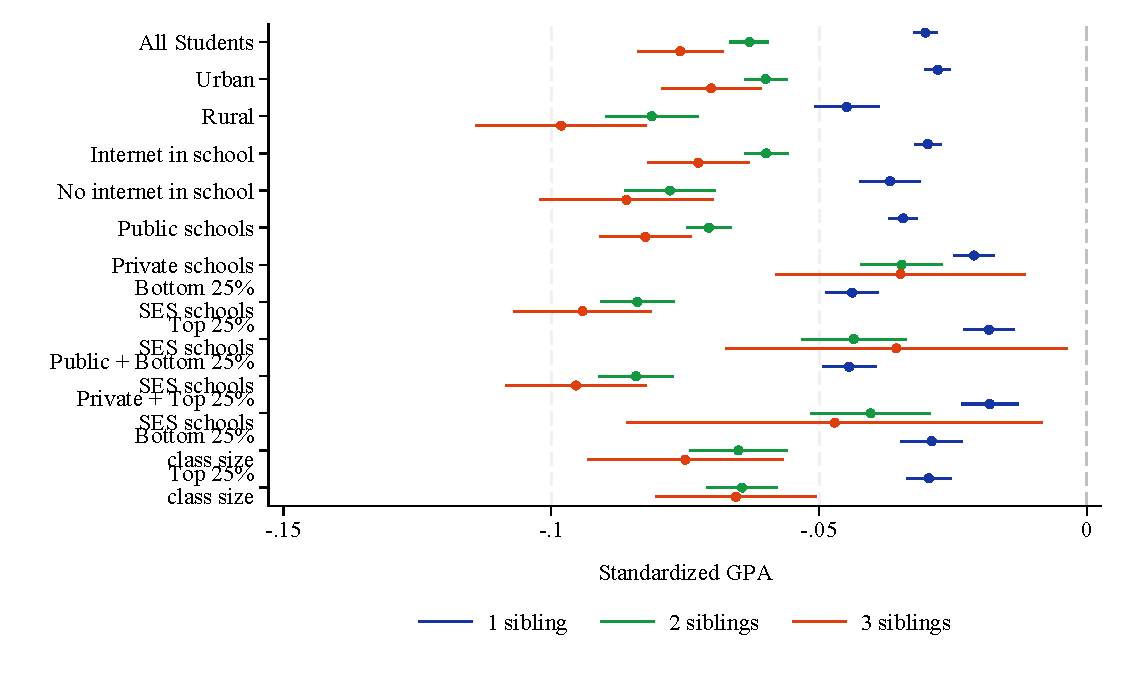
\includegraphics[width=\textwidth]{./FIGURES/TWFE/covid_twfe_A_bysibs_elm_all_gpa_m_adj_Tsiblings_Soldest_4.pdf}
        \caption{Change in gap between children with siblings and only childs}
        \label{fig:fig_appA}

\end{figure}

\begin{figure}[htbp]
    \centering
    
        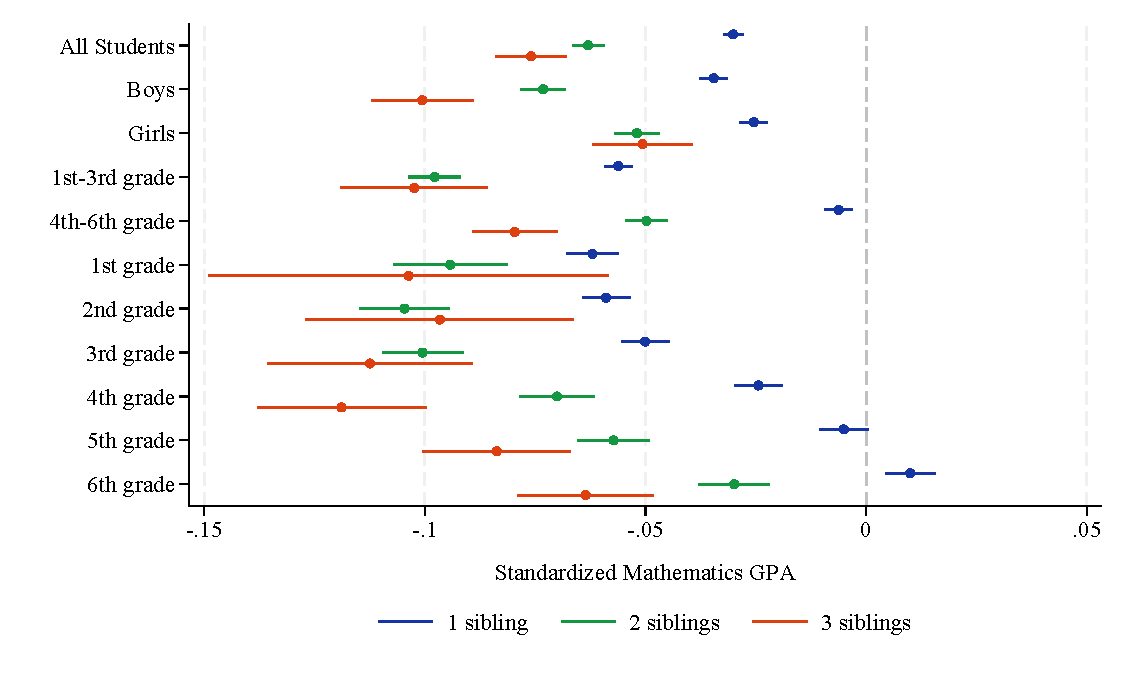
\includegraphics[width=\textwidth]{./FIGURES/TWFE/covid_twfe_B_bysibs_elm_all_gpa_m_adj_Tsiblings_Soldest_4.pdf}
        \caption{Change in gap between children with siblings and only childs}
        \label{fig:fig_appB}

\end{figure}

\begin{figure}[htbp]
    \centering
    
        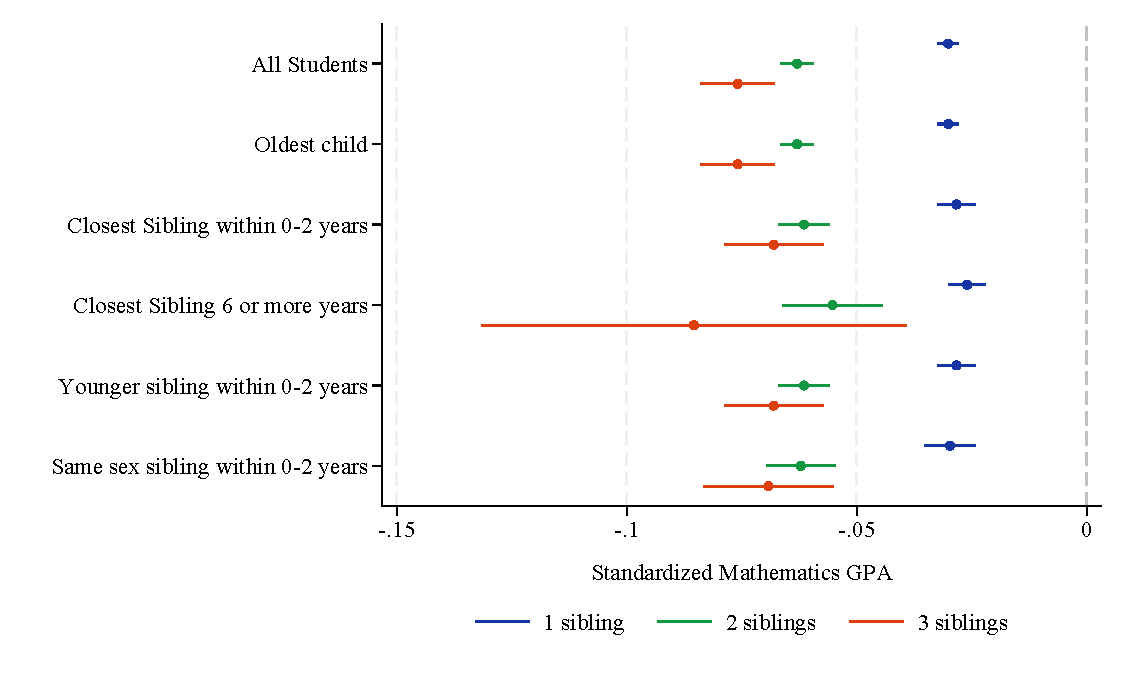
\includegraphics[width=\textwidth]{./FIGURES/TWFE/covid_twfe_C_bysibs_elm_all_gpa_m_adj_Tsiblings_Soldest_4.pdf}
        \caption{Change in gap between children with siblings and only childs}
        \label{fig:fig_appC}

\end{figure}


\begin{figure}[htbp]
    \centering
    
        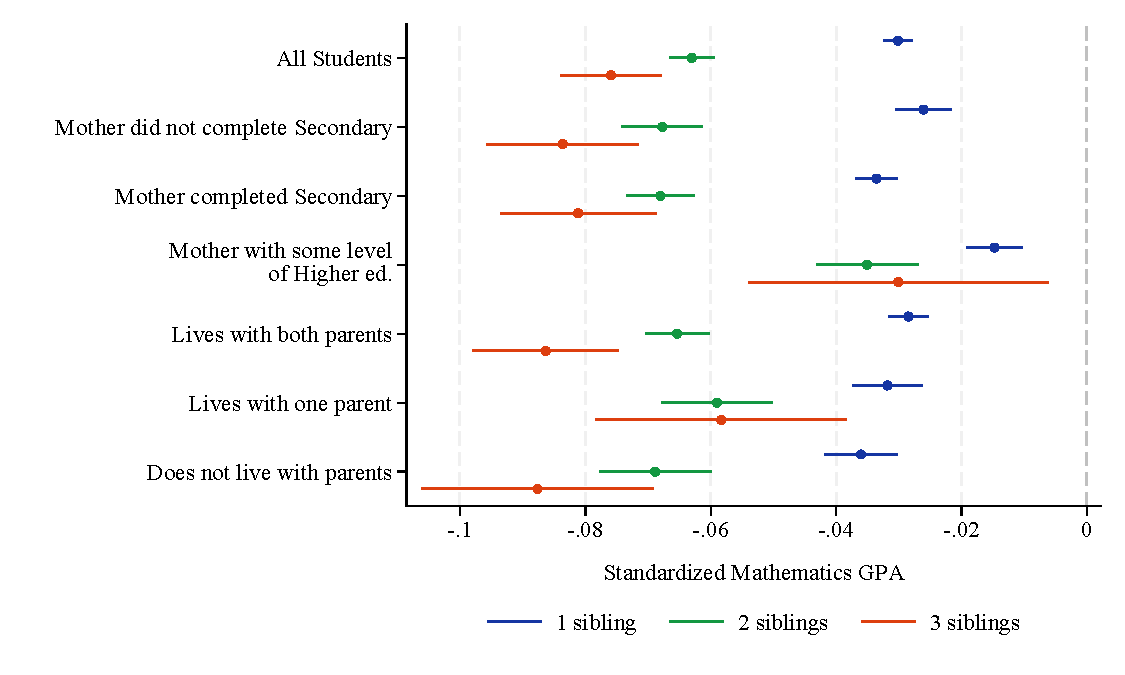
\includegraphics[width=\textwidth]{./FIGURES/TWFE/covid_twfe_D_bysibs_elm_all_gpa_m_adj_Tsiblings_Soldest_4.pdf}
        \caption{Change in gap between children with siblings and only childs}
        \label{fig:fig_appD}

\end{figure}



\makebox[0.1\width][l]{
\resizebox{\textwidth}{!}{
\begin{tabular}{lccc}
\toprule
\cmidrule(lr){2-4}
& \multicolumn{3}{c}{Standardized GPA}
\cmidrule(lr){2-4}
& Pre-Covid & Covid & Post-Covid  \\
& 2018-2019 & 2020-2021 & 2022-2023  \\
\cmidrule(lr){2-2} \cmidrule(lr){3-3} \cmidrule(lr){4-4}
& (1) & (2) & (3)  \\
\bottomrule
&  &  &   \\
Delay School (After SSA)&      -0.001   &      -0.010   &      -0.004   \\
                    &     (0.006)   &     (0.006)   &     (0.006)   \\
Local Linear        &         Yes   &         Yes   &         Yes   \\
                    &               &               &               \\
Observations        &     418,987   &     371,966   &     485,601   \\
Counterfactual mean &       0.043   &       0.020   &       0.031   \\
Bandwidth           &         365   &         365   &         365   \\
 

\bottomrule
\end{tabular}
}
}


\newpage

\makeatletter
\@ifclassloaded{beamer}{%
       \centering
       \resizebox{0.6\textwidth}{!}%
}{%
       \begin{table}[!tbp]\centering\def\sym#1{\ifmmode^{#1}\else\(^{#1}\)\fi}
       \centering
       \caption{Effects of younger sibling delaying school on older sibling standardized exams - 2 - m - a -  - 365}
       \label{tab:rd_summ_2_m_a_365}
       \resizebox{0.95\textwidth}{!}%
}
{
\makeatother
\makebox[0.1\width][l]{
\resizebox{\textwidth}{!}{
\begin{tabular}{lccc}
\toprule
\cmidrule(lr){2-4}
& \multicolumn{3}{c}{Standardized GPA} \\
\cmidrule(lr){2-4}
& Pre-Covid & Covid & Post-Covid  \\
& 2018-2019 & 2020-2021 & 2022-2023  \\
\cmidrule(lr){2-2} \cmidrule(lr){3-3} \cmidrule(lr){4-4}
& (1) & (2) & (3)  \\
\bottomrule
&  &  &   \\
\multirow{2}{*}{\shortstack[l]{Younger sibling born after \\ school-entry cutoff}}&      -0.000   &      -0.008   &       0.001   \\
                    &     (0.008)   &     (0.007)   &     (0.007)   \\
Local Linear        &         Yes   &         Yes   &         Yes   \\
                    &               &               &               \\
Observations        &     268,561   &     288,245   &     357,788   \\
Counterfactual mean &       0.053   &       0.027   &       0.053   \\
Bandwidth           &         365   &         365   &         365   \\
 

\bottomrule
\end{tabular}
}
\@ifclassloaded{beamer}{%
}{%
       \end{table}
}


\makeatletter
\@ifclassloaded{beamer}{%
       \centering
       \resizebox{0.6\textwidth}{!}%
}{%
       \begin{table}[!tbp]\centering\def\sym#1{\ifmmode^{#1}\else\(^{#1}\)\fi}
       \centering
       \caption{TWFE on GPA by baseline resources}
       \label{tab:twfe_ece_survey_1_pair1}
       \resizebox{0.65\textwidth}{!}%
}
{
\makeatother
\begin{tabular}{lccc}
\toprule
\cmidrule(lr){2-4}
& \multicolumn{3}{c}{TWFE} \\
\cmidrule(lr){2-4}
& 1 sibling & 2 siblings & 3 siblings  \\
\cmidrule(lr){2-2} \cmidrule(lr){3-3} \cmidrule(lr){4-4}
& (1) & (2) & (3)\\
\bottomrule
&  &  &  \\
&  &  &   \\
\multicolumn{4}{l}{\textit{Panel A: All studentes}} \\
\hspace{3mm}Mathematics&      -0.046***&      -0.078***&      -0.077** \\
                    &     (0.013)   &     (0.018)   &     (0.035)   \\
 
%&  &  &   \\
\hspace{3mm}Reading &      -0.023*  &      -0.035*  &      -0.072** \\
                    &     (0.013)   &     (0.018)   &     (0.035)   \\
                    &               &               &               \\
\hspace{3mm}Observations&     108,585   &      85,464   &      72,938   \\
 
&  &  &   \\
\multicolumn{4}{l}{\textit{Panel B: Low SES Households (Q1)}} \\
\hspace{3mm}Mathematics&      -0.026   &      -0.029   &      -0.166***\\
                    &     (0.026)   &     (0.033)   &     (0.057)   \\
 
%&  &  &   \\
\hspace{3mm}Reading &       0.001   &      -0.001   &      -0.133** \\
                    &     (0.026)   &     (0.034)   &     (0.058)   \\
                    &               &               &               \\
\hspace{3mm}Observations&      25,600   &      20,717   &      17,069   \\
 
&  &  &   \\
\multicolumn{4}{l}{\textit{Panel C: High SES Households (Q4)}} \\
\hspace{3mm}Mathematics&      -0.069** &       0.013   &       0.034   \\
                    &     (0.034)   &     (0.056)   &     (0.155)   \\
 
%&  &  &   \\
\hspace{3mm}Reading &      -0.026   &      -0.045   &       0.279*  \\
                    &     (0.034)   &     (0.056)   &     (0.153)   \\
                    &               &               &               \\
\hspace{3mm}Observations&      18,418   &      13,891   &      12,219   \\
 
&  &  &   \\
\multicolumn{4}{l}{\textit{Panel D: Households with no PC or Internet}} \\
\hspace{3mm}Mathematics&      -0.057***&      -0.113***&      -0.058   \\
                    &     (0.020)   &     (0.027)   &     (0.051)   \\
 
%&  &  &   \\
\hspace{3mm}Reading &      -0.036*  &      -0.033   &      -0.069   \\
                    &     (0.020)   &     (0.027)   &     (0.051)   \\
                    &               &               &               \\
\hspace{3mm}Observations&      46,281   &      36,305   &      30,041   \\
 
&  &  &   \\
\multicolumn{4}{l}{\textit{Panel E: Households with both PC and Internet}} \\
\hspace{3mm}Mathematics&      -0.013   &       0.015   &       0.307** \\
                    &     (0.034)   &     (0.056)   &     (0.146)   \\
 
%&  &  &   \\
\hspace{3mm}Reading &       0.009   &       0.006   &       0.505***\\
                    &     (0.035)   &     (0.056)   &     (0.147)   \\
                    &               &               &               \\
\hspace{3mm}Observations&      18,086   &      13,736   &      12,097   \\
 

\bottomrule
\end{tabular}
}
\@ifclassloaded{beamer}{%
}{%
       \end{table}
}

\makeatletter
\@ifclassloaded{beamer}{%
       \centering
       \resizebox{0.6\textwidth}{!}%
}{%
       \begin{table}[!tbp]\centering\def\sym#1{\ifmmode^{#1}\else\(^{#1}\)\fi}
       \centering
       \caption{TWFE on GPA by baseline resources}
       \label{tab:twfe_ece_survey_1_pair2}
       \resizebox{0.65\textwidth}{!}%
}
{
\makeatother
\begin{tabular}{lccc}
\toprule
\cmidrule(lr){2-4}
& \multicolumn{3}{c}{TWFE} \\
\cmidrule(lr){2-4}
& 1 sibling & 2 siblings & 3 siblings  \\
\cmidrule(lr){2-2} \cmidrule(lr){3-3} \cmidrule(lr){4-4}
& (1) & (2) & (3)\\
\bottomrule
&  &  &  \\
&  &  &   \\
\multicolumn{4}{l}{\textit{Panel A: All studentes}} \\
\hspace{3mm}Mathematics&      -0.024***&      -0.062***&      -0.110***\\
                    &     (0.007)   &     (0.010)   &     (0.019)   \\
 
%&  &  &   \\
\hspace{3mm}Reading &      -0.014** &      -0.064***&      -0.077***\\
                    &     (0.007)   &     (0.010)   &     (0.020)   \\
                    &               &               &               \\
\hspace{3mm}Observations&     341,265   &     272,263   &     236,637   \\
 
&  &  &   \\
\multicolumn{4}{l}{\textit{Panel B: Low SES Households (Q1)}} \\
\hspace{3mm}Mathematics&      -0.014   &      -0.048** &      -0.131***\\
                    &     (0.015)   &     (0.019)   &     (0.031)   \\
 
%&  &  &   \\
\hspace{3mm}Reading &      -0.004   &      -0.050***&      -0.073** \\
                    &     (0.015)   &     (0.019)   &     (0.031)   \\
                    &               &               &               \\
\hspace{3mm}Observations&      73,524   &      61,008   &      51,297   \\
 
&  &  &   \\
\multicolumn{4}{l}{\textit{Panel C: High SES Households (Q4)}} \\
\hspace{3mm}Mathematics&      -0.038** &      -0.041   &      -0.203***\\
                    &     (0.016)   &     (0.028)   &     (0.073)   \\
 
%&  &  &   \\
\hspace{3mm}Reading &      -0.029*  &      -0.047*  &      -0.043   \\
                    &     (0.016)   &     (0.028)   &     (0.074)   \\
                    &               &               &               \\
\hspace{3mm}Observations&      70,576   &      54,091   &      48,686   \\
 
&  &  &   \\
\multicolumn{4}{l}{\textit{Panel D: Households with no PC or Internet}} \\
\hspace{3mm}Mathematics&      -0.027*  &      -0.054** &      -0.084*  \\
                    &     (0.014)   &     (0.021)   &     (0.048)   \\
 
%&  &  &   \\
\hspace{3mm}Reading &      -0.015   &      -0.054***&      -0.057   \\
                    &     (0.014)   &     (0.021)   &     (0.048)   \\
                    &               &               &               \\
\hspace{3mm}Observations&     104,804   &      84,220   &      73,029   \\
 
&  &  &   \\
\multicolumn{4}{l}{\textit{Panel E: Households with both PC and Internet}} \\
\hspace{3mm}Mathematics&      -0.036***&      -0.032*  &      -0.144***\\
                    &     (0.012)   &     (0.019)   &     (0.041)   \\
 
%&  &  &   \\
\hspace{3mm}Reading &      -0.027** &      -0.051***&      -0.064   \\
                    &     (0.013)   &     (0.019)   &     (0.042)   \\
                    &               &               &               \\
\hspace{3mm}Observations&     125,843   &      98,884   &      85,077   \\
 

\bottomrule
\end{tabular}
}
\@ifclassloaded{beamer}{%
}{%
       \end{table}
}

\makeatletter
\@ifclassloaded{beamer}{%
       \centering
       \resizebox{0.6\textwidth}{!}%
}{%
       \begin{table}[!tbp]\centering\def\sym#1{\ifmmode^{#1}\else\(^{#1}\)\fi}
       \centering
       \caption{TWFE on 7th grade GPA by 4th grade baseline resources}
       \label{tab:twfe_gpa_baseline_survey_1_pair3}
       \resizebox{0.65\textwidth}{!}%
}
{
\makeatother
\begin{tabular}{lccc}
\toprule
\cmidrule(lr){2-4}
& \multicolumn{3}{c}{TWFE} \\
\cmidrule(lr){2-4}
& 1 sibling & 2 siblings & 3 siblings  \\
\cmidrule(lr){2-2} \cmidrule(lr){3-3} \cmidrule(lr){4-4}
& (1) & (2) & (3)\\
\bottomrule
&  &  &  \\
&  &  &   \\
\multicolumn{4}{l}{\textit{Panel A: All studentes}} \\
\hspace{3mm}Mathematics&      -0.024***&      -0.070***&      -0.060***\\
                    &     (0.007)   &     (0.010)   &     (0.018)   \\
 
%&  &  &   \\
\hspace{3mm}Reading &      -0.021***&      -0.045***&      -0.033*  \\
                    &     (0.007)   &     (0.010)   &     (0.018)   \\
                    &               &               &               \\
\hspace{3mm}Observations&     365,702   &     292,698   &     254,104   \\
 
&  &  &   \\
\multicolumn{4}{l}{\textit{Panel B: Low SES Households (Q1)}} \\
\hspace{3mm}Mathematics&      -0.000   &      -0.020   &      -0.005   \\
                    &     (0.014)   &     (0.017)   &     (0.028)   \\
 
%&  &  &   \\
\hspace{3mm}Reading &      -0.012   &      -0.006   &       0.004   \\
                    &     (0.014)   &     (0.017)   &     (0.028)   \\
                    &               &               &               \\
\hspace{3mm}Observations&      90,252   &      75,485   &      63,910   \\
 
&  &  &   \\
\multicolumn{4}{l}{\textit{Panel C: High SES Households (Q4)}} \\
\hspace{3mm}Mathematics&      -0.026*  &      -0.091***&      -0.106   \\
                    &     (0.016)   &     (0.027)   &     (0.071)   \\
 
%&  &  &   \\
\hspace{3mm}Reading &      -0.031** &      -0.097***&      -0.066   \\
                    &     (0.016)   &     (0.027)   &     (0.072)   \\
                    &               &               &               \\
\hspace{3mm}Observations&      73,259   &      56,234   &      50,652   \\
 
&  &  &   \\
\multicolumn{4}{l}{\textit{Panel D: Households with no PC or Internet}} \\
\hspace{3mm}Mathematics&      -0.018   &      -0.107***&      -0.084*  \\
                    &     (0.013)   &     (0.020)   &     (0.046)   \\
 
%&  &  &   \\
\hspace{3mm}Reading &      -0.021   &      -0.077***&      -0.107** \\
                    &     (0.013)   &     (0.020)   &     (0.047)   \\
                    &               &               &               \\
\hspace{3mm}Observations&     113,464   &      91,731   &      79,607   \\
 
&  &  &   \\
\multicolumn{4}{l}{\textit{Panel E: Households with both PC and Internet}} \\
\hspace{3mm}Mathematics&      -0.007   &      -0.023   &      -0.003   \\
                    &     (0.012)   &     (0.018)   &     (0.040)   \\
 
%&  &  &   \\
\hspace{3mm}Reading &       0.006   &      -0.030*  &      -0.016   \\
                    &     (0.012)   &     (0.018)   &     (0.040)   \\
                    &               &               &               \\
\hspace{3mm}Observations&     136,957   &     108,035   &      92,888   \\
 

\bottomrule
\end{tabular}
}
\@ifclassloaded{beamer}{%
}{%
       \end{table}
}

\makeatletter
\@ifclassloaded{beamer}{%
       \centering
       \resizebox{0.6\textwidth}{!}%
}{%
       \begin{table}[!tbp]\centering\def\sym#1{\ifmmode^{#1}\else\(^{#1}\)\fi}
       \centering
       \caption{TWFE on GPA by baseline resources}
       \label{tab:twfe_ece_survey_1_pair4}
       \resizebox{0.65\textwidth}{!}%
}
{
\makeatother
\begin{tabular}{lccc}
\toprule
\cmidrule(lr){2-4}
& \multicolumn{3}{c}{TWFE} \\
\cmidrule(lr){2-4}
& 1 sibling & 2 siblings & 3 siblings  \\
\cmidrule(lr){2-2} \cmidrule(lr){3-3} \cmidrule(lr){4-4}
& (1) & (2) & (3)\\
\bottomrule
&  &  &  \\
&  &  &   \\
\multicolumn{4}{l}{\textit{Panel A: All studentes}} \\
\hspace{3mm}Mathematics&      -0.032***&      -0.053***&      -0.074***\\
                    &     (0.006)   &     (0.008)   &     (0.014)   \\
 
%&  &  &   \\
\hspace{3mm}Reading &      -0.018***&      -0.035***&      -0.045***\\
                    &     (0.006)   &     (0.008)   &     (0.014)   \\
                    &               &               &               \\
\hspace{3mm}Observations&     466,128   &     384,809   &     339,142   \\
 
&  &  &   \\
\multicolumn{4}{l}{\textit{Panel B: Low SES Households (Q1)}} \\
\hspace{3mm}Mathematics&      -0.018   &      -0.023   &      -0.044** \\
                    &     (0.012)   &     (0.015)   &     (0.021)   \\
 
%&  &  &   \\
\hspace{3mm}Reading &      -0.002   &      -0.006   &      -0.045** \\
                    &     (0.012)   &     (0.015)   &     (0.022)   \\
                    &               &               &               \\
\hspace{3mm}Observations&     119,170   &     103,085   &      90,231   \\
 
&  &  &   \\
\multicolumn{4}{l}{\textit{Panel C: High SES Households (Q4)}} \\
\hspace{3mm}Mathematics&      -0.039***&      -0.074***&      -0.091*  \\
                    &     (0.013)   &     (0.021)   &     (0.050)   \\
 
%&  &  &   \\
\hspace{3mm}Reading &      -0.026*  &      -0.057***&      -0.027   \\
                    &     (0.013)   &     (0.022)   &     (0.050)   \\
                    &               &               &               \\
\hspace{3mm}Observations&      91,916   &      72,508   &      64,890   \\
 
&  &  &   \\
\multicolumn{4}{l}{\textit{Panel D: Households with no PC or Internet}} \\
\hspace{3mm}Mathematics&      -0.032***&      -0.059***&      -0.063** \\
                    &     (0.009)   &     (0.014)   &     (0.029)   \\
 
%&  &  &   \\
\hspace{3mm}Reading &      -0.021** &      -0.036** &       0.004   \\
                    &     (0.010)   &     (0.014)   &     (0.030)   \\
                    &               &               &               \\
\hspace{3mm}Observations&     186,154   &     149,785   &     133,378   \\
 
&  &  &   \\
\multicolumn{4}{l}{\textit{Panel E: Households with both PC and Internet}} \\
\hspace{3mm}Mathematics&      -0.031***&      -0.042***&      -0.095***\\
                    &     (0.010)   &     (0.013)   &     (0.020)   \\
 
%&  &  &   \\
\hspace{3mm}Reading &      -0.005   &      -0.030** &      -0.066***\\
                    &     (0.011)   &     (0.013)   &     (0.021)   \\
                    &               &               &               \\
\hspace{3mm}Observations&     153,436   &     130,307   &     113,257   \\
 

\bottomrule
\end{tabular}
}
\@ifclassloaded{beamer}{%
}{%
       \end{table}
}


\makeatletter
\@ifclassloaded{beamer}{%
       \centering
       \resizebox{0.6\textwidth}{!}%
}{%
       \begin{table}[!tbp]\centering\def\sym#1{\ifmmode^{#1}\else\(^{#1}\)\fi}
       \centering
       \caption{TWFE on 6th grade GPA by 2nd grade baseline achievement and expectations}
       \label{tab:twfe_gpa_baseline_survey_2_pair1}
       \resizebox{0.65\textwidth}{!}%
}
{
\makeatother
\begin{tabular}{lccc}
\toprule
\cmidrule(lr){2-4}
& \multicolumn{3}{c}{TWFE} \\
\cmidrule(lr){2-4}
& 1 sibling & 2 siblings & 3 siblings  \\
\cmidrule(lr){2-2} \cmidrule(lr){3-3} \cmidrule(lr){4-4}
& (1) & (2) & (3)\\
\bottomrule
&  &  &  \\
&  &  &   \\
\multicolumn{4}{l}{\textit{Panel A: All studentes}} \\
\hspace{3mm}Mathematics&      -0.046***&      -0.078***&      -0.077** \\
                    &     (0.013)   &     (0.018)   &     (0.035)   \\
 
%&  &  &   \\
\hspace{3mm}Reading &      -0.023*  &      -0.035*  &      -0.072** \\
                    &     (0.013)   &     (0.018)   &     (0.035)   \\
                    &               &               &               \\
\hspace{3mm}Observations&     108,585   &      85,464   &      72,938   \\
 
&  &  &   \\
\multicolumn{4}{l}{\textit{Panel B: Student in bottom quartile of achievement}} \\
\hspace{3mm}Mathematics&      -0.028   &      -0.073*  &      -0.160** \\
                    &     (0.032)   &     (0.041)   &     (0.072)   \\
 
%&  &  &   \\
\hspace{3mm}Reading &       0.018   &      -0.026   &      -0.095   \\
                    &     (0.032)   &     (0.042)   &     (0.073)   \\
                    &               &               &               \\
\hspace{3mm}Observations&      14,632   &      11,987   &      10,145   \\
 
&  &  &   \\
\multicolumn{4}{l}{\textit{Panel C: Student in top quartile of achievement}} \\
\hspace{3mm}Mathematics&      -0.061** &      -0.103***&       0.030   \\
                    &     (0.026)   &     (0.038)   &     (0.083)   \\
 
%&  &  &   \\
\hspace{3mm}Reading &      -0.049*  &      -0.044   &       0.009   \\
                    &     (0.026)   &     (0.038)   &     (0.084)   \\
                    &               &               &               \\
\hspace{3mm}Observations&      34,500   &      26,134   &      22,113   \\
 
&  &  &   \\
\multicolumn{4}{l}{\textit{Panel D: Max Expectation: Finish school}} \\
\hspace{3mm}Mathematics&       0.004   &      -0.078   &      -0.222   \\
                    &     (0.063)   &     (0.083)   &     (0.141)   \\
 
%&  &  &   \\
\hspace{3mm}Reading &       0.037   &       0.004   &      -0.250*  \\
                    &     (0.064)   &     (0.085)   &     (0.145)   \\
                    &               &               &               \\
\hspace{3mm}Observations&       5,127   &       4,075   &       3,422   \\
 
&  &  &   \\
\multicolumn{4}{l}{\textit{Panel E: Max Expectation: 4-year college or grad school}} \\
\hspace{3mm}Mathematics&      -0.048***&      -0.073***&      -0.041   \\
                    &     (0.015)   &     (0.021)   &     (0.042)   \\
 
%&  &  &   \\
\hspace{3mm}Reading &      -0.030** &      -0.031   &      -0.041   \\
                    &     (0.015)   &     (0.021)   &     (0.043)   \\
                    &               &               &               \\
\hspace{3mm}Observations&      87,535   &      67,871   &      57,831   \\
 

\bottomrule
\end{tabular}
}
\@ifclassloaded{beamer}{%
}{%
       \end{table}
}

\makeatletter
\@ifclassloaded{beamer}{%
       \centering
       \resizebox{0.6\textwidth}{!}%
}{%
       \begin{table}[!tbp]\centering\def\sym#1{\ifmmode^{#1}\else\(^{#1}\)\fi}
       \centering
       \caption{TWFE on 6th grade GPA by 4th grade baseline achievement and expectations}
       \label{tab:twfe_gpa_baseline_survey_2_pair2}
       \resizebox{0.65\textwidth}{!}%
}
{
\makeatother
\begin{tabular}{lccc}
\toprule
\cmidrule(lr){2-4}
& \multicolumn{3}{c}{TWFE} \\
\cmidrule(lr){2-4}
& 1 sibling & 2 siblings & 3 siblings  \\
\cmidrule(lr){2-2} \cmidrule(lr){3-3} \cmidrule(lr){4-4}
& (1) & (2) & (3)\\
\bottomrule
&  &  &  \\
&  &  &   \\
\multicolumn{4}{l}{\textit{Panel A: All studentes}} \\
\hspace{3mm}Mathematics&      -0.024***&      -0.062***&      -0.110***\\
                    &     (0.007)   &     (0.010)   &     (0.019)   \\
 
%&  &  &   \\
\hspace{3mm}Reading &      -0.014** &      -0.064***&      -0.077***\\
                    &     (0.007)   &     (0.010)   &     (0.020)   \\
                    &               &               &               \\
\hspace{3mm}Observations&     341,265   &     272,263   &     236,637   \\
 
&  &  &   \\
\multicolumn{4}{l}{\textit{Panel B: Student in bottom quartile of achievement}} \\
\hspace{3mm}Mathematics&      -0.013   &      -0.052***&      -0.084** \\
                    &     (0.015)   &     (0.020)   &     (0.035)   \\
 
%&  &  &   \\
\hspace{3mm}Reading &      -0.005   &      -0.049** &      -0.078** \\
                    &     (0.015)   &     (0.020)   &     (0.035)   \\
                    &               &               &               \\
\hspace{3mm}Observations&      64,124   &      52,974   &      45,942   \\
 
&  &  &   \\
\multicolumn{4}{l}{\textit{Panel C: Student in top quartile of achievement}} \\
\hspace{3mm}Mathematics&      -0.038** &      -0.094***&      -0.098** \\
                    &     (0.015)   &     (0.022)   &     (0.048)   \\
 
%&  &  &   \\
\hspace{3mm}Reading &      -0.022   &      -0.071***&      -0.095*  \\
                    &     (0.015)   &     (0.023)   &     (0.049)   \\
                    &               &               &               \\
\hspace{3mm}Observations&      97,944   &      74,571   &      64,319   \\
 
&  &  &   \\
\multicolumn{4}{l}{\textit{Panel D: Max Expectation: Finish school}} \\
\hspace{3mm}Mathematics&      -0.021   &      -0.064*  &       0.062   \\
                    &     (0.030)   &     (0.039)   &     (0.065)   \\
 
%&  &  &   \\
\hspace{3mm}Reading &      -0.004   &      -0.082** &      -0.018   \\
                    &     (0.030)   &     (0.039)   &     (0.065)   \\
                    &               &               &               \\
\hspace{3mm}Observations&      22,087   &      18,509   &      15,822   \\
 
&  &  &   \\
\multicolumn{4}{l}{\textit{Panel E: Max Expectation: 4-year college or grad school}} \\
\hspace{3mm}Mathematics&      -0.028***&      -0.061***&      -0.136***\\
                    &     (0.008)   &     (0.012)   &     (0.024)   \\
 
%&  &  &   \\
\hspace{3mm}Reading &      -0.018** &      -0.062***&      -0.106***\\
                    &     (0.008)   &     (0.012)   &     (0.024)   \\
                    &               &               &               \\
\hspace{3mm}Observations&     270,591   &     212,753   &     184,893   \\
 

\bottomrule
\end{tabular}
}
\@ifclassloaded{beamer}{%
}{%
       \end{table}
}

\makeatletter
\@ifclassloaded{beamer}{%
       \centering
       \resizebox{0.6\textwidth}{!}%
}{%
       \begin{table}[!tbp]\centering\def\sym#1{\ifmmode^{#1}\else\(^{#1}\)\fi}
       \centering
       \caption{WFE on GPA by baseline achievement and expectations}
       \label{tab:twfe_gpa_baseline_survey_2_pair3}
       \resizebox{0.65\textwidth}{!}%
}
{
\makeatother
\begin{tabular}{lccc}
\toprule
\cmidrule(lr){2-4}
& \multicolumn{3}{c}{TWFE} \\
\cmidrule(lr){2-4}
& 1 sibling & 2 siblings & 3 siblings  \\
\cmidrule(lr){2-2} \cmidrule(lr){3-3} \cmidrule(lr){4-4}
& (1) & (2) & (3)\\
\bottomrule
&  &  &  \\
&  &  &   \\
\multicolumn{4}{l}{\textit{Panel A: All studentes}} \\
\hspace{3mm}Mathematics&      -0.024***&      -0.070***&      -0.060***\\
                    &     (0.007)   &     (0.010)   &     (0.018)   \\
 
%&  &  &   \\
\hspace{3mm}Reading &      -0.021***&      -0.045***&      -0.033*  \\
                    &     (0.007)   &     (0.010)   &     (0.018)   \\
                    &               &               &               \\
\hspace{3mm}Observations&     365,702   &     292,698   &     254,104   \\
 
&  &  &   \\
\multicolumn{4}{l}{\textit{Panel B: Student in bottom quartile of achievement}} \\
\hspace{3mm}Mathematics&       0.022   &      -0.009   &      -0.101***\\
                    &     (0.015)   &     (0.019)   &     (0.033)   \\
 
%&  &  &   \\
\hspace{3mm}Reading &       0.020   &      -0.005   &      -0.015   \\
                    &     (0.015)   &     (0.020)   &     (0.034)   \\
                    &               &               &               \\
\hspace{3mm}Observations&      76,396   &      63,590   &      55,311   \\
 
&  &  &   \\
\multicolumn{4}{l}{\textit{Panel C: Student in top quartile of achievement}} \\
\hspace{3mm}Mathematics&      -0.046***&      -0.118***&      -0.166***\\
                    &     (0.014)   &     (0.021)   &     (0.045)   \\
 
%&  &  &   \\
\hspace{3mm}Reading &      -0.042***&      -0.081***&      -0.062   \\
                    &     (0.014)   &     (0.021)   &     (0.045)   \\
                    &               &               &               \\
\hspace{3mm}Observations&     100,921   &      76,928   &      66,386   \\
 
&  &  &   \\
\multicolumn{4}{l}{\textit{Panel D: Max Expectation: Finish school}} \\
\hspace{3mm}Mathematics&       0.018   &      -0.033   &      -0.035   \\
                    &     (0.029)   &     (0.037)   &     (0.060)   \\
 
%&  &  &   \\
\hspace{3mm}Reading &      -0.085***&      -0.057   &      -0.051   \\
                    &     (0.029)   &     (0.037)   &     (0.060)   \\
                    &               &               &               \\
\hspace{3mm}Observations&      26,308   &      22,144   &      19,072   \\
 
&  &  &   \\
\multicolumn{4}{l}{\textit{Panel E: Max Expectation: 4-year college or grad school}} \\
\hspace{3mm}Mathematics&      -0.032***&      -0.087***&      -0.092***\\
                    &     (0.008)   &     (0.011)   &     (0.022)   \\
 
%&  &  &   \\
\hspace{3mm}Reading &      -0.024***&      -0.057***&      -0.076***\\
                    &     (0.008)   &     (0.011)   &     (0.023)   \\
                    &               &               &               \\
\hspace{3mm}Observations&     287,508   &     226,685   &     196,682   \\
 

\bottomrule
\end{tabular}
}
\@ifclassloaded{beamer}{%
}{%
       \end{table}
}

\makeatletter
\@ifclassloaded{beamer}{%
       \centering
       \resizebox{0.6\textwidth}{!}%
}{%
       \begin{table}[!tbp]\centering\def\sym#1{\ifmmode^{#1}\else\(^{#1}\)\fi}
       \centering
       \caption{TWFE on 9th grade GPA by 8th grade baseline achievement and expectations}
       \label{tab:twfe_gpa_baseline_survey_2_pair4}
       \resizebox{0.65\textwidth}{!}%
}
{
\makeatother
\begin{tabular}{lccc}
\toprule
\cmidrule(lr){2-4}
& \multicolumn{3}{c}{TWFE} \\
\cmidrule(lr){2-4}
& 1 sibling & 2 siblings & 3 siblings  \\
\cmidrule(lr){2-2} \cmidrule(lr){3-3} \cmidrule(lr){4-4}
& (1) & (2) & (3)\\
\bottomrule
&  &  &  \\
&  &  &   \\
\multicolumn{4}{l}{\textit{Panel A: All studentes}} \\
\hspace{3mm}Mathematics&      -0.032***&      -0.053***&      -0.074***\\
                    &     (0.006)   &     (0.008)   &     (0.014)   \\
 
%&  &  &   \\
\hspace{3mm}Reading &      -0.018***&      -0.035***&      -0.045***\\
                    &     (0.006)   &     (0.008)   &     (0.014)   \\
                    &               &               &               \\
\hspace{3mm}Observations&     466,128   &     384,809   &     339,142   \\
 
&  &  &   \\
\multicolumn{4}{l}{\textit{Panel B: Student in bottom quartile of achievement}} \\
\hspace{3mm}Mathematics&       0.001   &      -0.043***&      -0.104***\\
                    &     (0.012)   &     (0.015)   &     (0.023)   \\
 
%&  &  &   \\
\hspace{3mm}Reading &       0.012   &      -0.049***&      -0.079***\\
                    &     (0.012)   &     (0.016)   &     (0.024)   \\
                    &               &               &               \\
\hspace{3mm}Observations&     100,937   &      86,703   &      76,726   \\
 
&  &  &   \\
\multicolumn{4}{l}{\textit{Panel C: Student in top quartile of achievement}} \\
\hspace{3mm}Mathematics&      -0.062***&      -0.100***&      -0.171***\\
                    &     (0.012)   &     (0.018)   &     (0.037)   \\
 
%&  &  &   \\
\hspace{3mm}Reading &      -0.030** &      -0.065***&      -0.091** \\
                    &     (0.012)   &     (0.018)   &     (0.037)   \\
                    &               &               &               \\
\hspace{3mm}Observations&     127,522   &     100,695   &      88,372   \\
 
&  &  &   \\
\multicolumn{4}{l}{\textit{Panel D: Max Expectation: Finish school}} \\
\hspace{3mm}Mathematics&       0.028   &       0.033   &      -0.071   \\
                    &     (0.025)   &     (0.032)   &     (0.052)   \\
 
%&  &  &   \\
\hspace{3mm}Reading &       0.017   &       0.060*  &      -0.031   \\
                    &     (0.026)   &     (0.034)   &     (0.056)   \\
                    &               &               &               \\
\hspace{3mm}Observations&      25,985   &      21,700   &      18,777   \\
 
&  &  &   \\
\multicolumn{4}{l}{\textit{Panel E: Max Expectation: 4-year college or grad school}} \\
\hspace{3mm}Mathematics&      -0.036***&      -0.061***&      -0.084***\\
                    &     (0.007)   &     (0.009)   &     (0.016)   \\
 
%&  &  &   \\
\hspace{3mm}Reading &      -0.019***&      -0.043***&      -0.059***\\
                    &     (0.007)   &     (0.009)   &     (0.016)   \\
                    &               &               &               \\
\hspace{3mm}Observations&     389,469   &     319,269   &     281,150   \\
 

\bottomrule
\end{tabular}
}
\@ifclassloaded{beamer}{%
}{%
       \end{table}
}




\clearpage

\setcounter{figure}{0}
\renewcommand\thefigure{B.\arabic{figure}}    

\setcounter{table}{0}
\renewcommand{\thetable}{B.\arabic{table}}
\setcounter{subsection}{0}

\section*{Appendix B: Robustness} \label{sec:appB}

%\section{Robustness}\label{sec:robustness}

\subsection{Potential sample selection}

Discuss how siblings are observed. We only see observations as long as they are enrolled in data. Most children are enrolled in primary school \textcolor{green}{(show data from household surveys)}. However, most children are not enrolled until 3-4 years old. Since our last year of administrative data is 2024, this means that some families with 2 children, one of which was born after 2021, might be observed as only childs. To address any concerns from this selection I do the following:

\begin{itemize}
    \item These families are not particularly different from others? (this true)?
    \item I use data up to 2023 and 2022 to define families (and potentially imposing a similar bias to earlier years) and still see results change around COVID. \textcolor{green}{Pending Analyis}
\end{itemize}


\subsection{Siblings in same vs different schools}

\subsection{Different definitions of siblings: father, both, caretaker}

\subsection{Only children: Missreport}

What if they are mostly students leaving by themselves? And not reporting parent's IDs? How can we validate this?

\subsection{Younger and middle child}

\subsection{Unadjusted scores}


\clearpage


\setcounter{figure}{0}
\renewcommand\thefigure{C.\arabic{figure}}    

\setcounter{table}{0}
\renewcommand{\thetable}{C.\arabic{table}}
\setcounter{subsection}{0}

\section*{Appendix C: Heterogeneity} \label{sec:appC}

Surprisingly, results are consistent across...

\subsection{Reinforcement vs Compensation}



\clearpage

\setcounter{figure}{0}
\renewcommand\thefigure{D.\arabic{figure}}    

\setcounter{table}{0}
\renewcommand{\thetable}{D.\arabic{table}}
\setcounter{subsection}{0}

\section*{Appendix D: Validating Sibling Identification} \label{sec:appD}

\subsection{Contrasting with survey responses}


\subsection{Number of siblings}

In \textcolor{green}{XX} one survey question asked about number of siblings.


\subsection{Number of people in the household}

In the 2nd grade survey in 2015 and 2016 a question asked about the number of adults and children in the household. In \textcolor{green}{XX} I show the distribution of responses by number of children estimated with matching parent IDs. 

\subsection{Potential composition of sample}

By using older siblings, it is less and less likely to see them in lower grades for later years. For example, to see an older sibling with 3 younger siblings in 2024 in first grade, they would have to have siblings within 3 years below them, otherwise they wouldn't be seen in the data. These creates two isses. First, the TWFE might be overweighting school closure years over years after schools re-opened. We address this with the time fixed effect. Another issue is that these families are likely different given the short age gap between all the children. However, this issue is less prevalent in later grades. The fact that I see similar pattern in 1st as in 6th grade assuages concerns for this.


\setcounter{figure}{0}
\renewcommand\thefigure{I.\arabic{figure}}    

\setcounter{table}{0}
\renewcommand{\thetable}{I.\arabic{table}}
\setcounter{subsection}{0}

\clearpage

\section*{Appendix I: Issues to resolve} \label{sec:appI}

\subsection{Administrative data vs survey data}

In some years, we can compare administrative with survey data:

\textbf{Mother's education}: \hyperref[tab:survey_educ]{Table \ref{tab:survey_educ}}
This variable compares relatively well. 

\textbf{Family members}: \hyperref[tab:survey_siblings]{Table \ref{tab:survey_siblings}}
There are significant discrepancies in this variables. Only children report having no siblings more often than the other groups although at low rates (10\% vs 1\%) and less often living with siblings (74\% vs 90\%). However, the average number of siblings and household members shows no difference between the first two groups. When looking at family members they live with, the administrative data information does not accurately predict living conditions. \hyperref[tab:survey_living]{Table \ref{tab:survey_living}}. However, the admin data about living with their mother seems to be more precise than that of living with their father. Probably better to use 'lives with mother/doesnt live with mother' categories?

\makeatletter
\@ifclassloaded{beamer}{%
       \centering
       \resizebox{0.7\textwidth}{!}%
}{%
       \begin{table}[!tbp]\centering\def\sym#1{\ifmmode^{#1}\else\(^{#1}\)\fi}
       \centering
       \caption{Descriptive Statistics}
       \label{tab:survey_educ}
       \resizebox{0.8\textwidth}{!}%
}
{
\makeatother
\begin{tabular}{lccc}
\toprule
& No secondary education & Complete secondary & Higher education \\
\cmidrule(lr){2-2} \cmidrule(lr){3-3} \cmidrule(lr){4-4} 
& (1) & (2) & (3) \\
\bottomrule
&  &  &  \\

\multicolumn{4}{l}{\textit{Panel A: Survey vs Administrative data}} \\
            &            &            &                        \\
Did not complete secondary education & 0.745 & 0.248 & 0.040 \\
Completed secondary education & 0.188 & 0.456 & 0.147 \\
Some level of higher education & 0.067 & 0.295 & 0.813 \\            
\\
%\multicolumn{4}{l}{\textit{Panel B: Academic characteristics}} \\
            &            &            &                       \\
%\% Grade promotion&       0.931&       0.952&       0.934&       0.897\\

\bottomrule
\end{tabular}
}
\@ifclassloaded{beamer}{%
}{%
       \end{table}
}

%\makeatletter
\@ifclassloaded{beamer}{%
       \centering
       \resizebox{0.5\textwidth}{!}%
}{%
       \begin{table}[!tbp]\centering\def\sym#1{\ifmmode^{#1}\else\(^{#1}\)\fi}
       \centering
       \caption{Descriptive Statistics}
       \label{tab:descriptive}
       \resizebox{0.8\textwidth}{!}%
}
{
\makeatother
\begin{tabular}{lcccc}
\toprule
\cmidrule(lr){2-4}
& \multicolumn{4}{c}{TWFE}  \\
\cmidrule(lr){2-4}
& Only children & 1 sibling & 2 siblings & 3 siblings  \\
\cmidrule(lr){2-2} \cmidrule(lr){3-3} \cmidrule(lr){4-4} \cmidrule(lr){5-5}
& (1) & (2) & (3) & (4)\\
\bottomrule
&  &  &  & \\
&  &  &   \\
\multicolumn{4}{l}{\textit{Panel A: School and student characteristics}} \\
            &            &            &            &            \\
\% Urban    &       0.812&       0.814&       0.752&       0.645\\
\% Public School&       0.681&       0.702&       0.793&       0.879\\
Average Grade&       6.072&       5.952&       6.460&       6.910\\
\% Male     &       0.511&       0.512&       0.510&       0.506\\
&  &  &   \\
\multicolumn{4}{l}{\textit{Panel B: Academic characteristics}} \\
            &            &            &            &            \\
\% Grade promotion&       0.953&       0.963&       0.947&       0.920\\
\% Grade promotion without recovery&       0.826&       0.842&       0.799&       0.753\\
Standardized GPA (Mathematics) &       0.016&       0.072&       0.006&      -0.073\\
Standardized GPA (Reading)&       0.022&       0.071&      -0.001&      -0.083\\
&  &  &   \\
\multicolumn{4}{l}{\textit{Panel C: Parent's characteristics}} \\
            &            &            &            &            \\
\% Lives with both parents&       0.493&       0.558&       0.555&       0.536\\
\% Lives with one parent&       0.178&       0.170&       0.178&       0.179\\
\% Lives with Mother&       0.768&       0.768&       0.766&       0.747\\
\% Lives with Father&       0.670&       0.700&       0.694&       0.682\\
\% Father without complete secondary&       0.302&       0.272&       0.355&       0.490\\
\% Father with complete secondary&       0.428&       0.443&       0.428&       0.377\\
\% Father with some level of higher ed.&       0.270&       0.286&       0.217&       0.133\\
\% Father without complete secondary&       0.343&       0.323&       0.421&       0.569\\
\% Father with complete secondary&       0.413&       0.425&       0.401&       0.334\\
\% Father with some level of higher ed.&       0.244&       0.252&       0.179&       0.097\\
&  &  &   \\
\multicolumn{4}{l}{\textit{Panel D: Household Resources (2nd grade: 2015, 2016)}} \\
            &            &            &            &            \\
SES         &       0.122&       0.079&      -0.114&      -0.378\\
HH size     &       4.949&       5.035&       5.435&       5.876\\
\# of bedrooms&       2.846&       2.664&       2.604&       2.661\\
\% Radio    &       0.683&       0.653&       0.690&       0.704\\
\% Internet &       0.416&       0.415&       0.345&       0.243\\
\% PC       &       0.454&       0.458&       0.365&       0.258\\
\% Laptop   &       0.405&       0.412&       0.338&       0.242\\
\% 6+ books &       0.574&       0.527&       0.457&       0.377\\
\% Quiet room to study&       0.861&       0.855&       0.829&       0.796\\
&  &  &   \\
\multicolumn{4}{l}{\textit{Panel E: Academic Performance (2nd grade: 2015, 2016)}} \\
            &            &            &            &            \\
standardized Reading score&       0.702&       0.756&       0.621&       0.397\\
standardized Mathematics score&       0.608&       0.691&       0.570&       0.361\\
Did 3 years of Pre-K&       0.660&       0.668&       0.645&       0.572\\
Has repeated a grade&       0.035&       0.027&       0.037&       0.058\\
&  &  &   \\
\multicolumn{4}{l}{\textit{Panel F: Parent's Characteristics (2nd grade: 2015, 2016)}} \\
            &            &            &            &            \\
\% Mother with complete secondary&       0.251&       0.278&       0.279&       0.266\\
\% Mother with 4-year college&       0.398&       0.415&       0.318&       0.193\\
\% Spanish  &       0.866&       0.861&       0.847&       0.828\\
\%Education expectation: High School&       0.084&       0.071&       0.100&       0.159\\
\%Education expectation: 4-year college&       0.808&       0.828&       0.769&       0.671\\

\bottomrule
\end{tabular}
}
\@ifclassloaded{beamer}{%
}{%
       \end{table}
}

\makeatletter
\@ifclassloaded{beamer}{%
       \centering
       \resizebox{0.7\textwidth}{!}%
}{%
       \begin{table}[!tbp]\centering\def\sym#1{\ifmmode^{#1}\else\(^{#1}\)\fi}
       \centering
       \caption{Descriptive Statistics}
       \label{tab:survey_siblings}
       \resizebox{0.8\textwidth}{!}%
}
{
\makeatother
\begin{tabular}{lcccc}
\toprule
& Only children & 1 sibling & 2 siblings & 3 siblings  \\
\cmidrule(lr){2-2} \cmidrule(lr){3-3} \cmidrule(lr){4-4} \cmidrule(lr){5-5}
& (1) & (2) & (3) & (4)\\
\bottomrule
&  &  &  & \\

\multicolumn{4}{l}{\textit{Panel A: Survey vs Administrative data (8th grade)}} \\
            &            &            &            &            \\
\% no siblings in survey    & .102      & .01 & .006 & .005 \\
\% lives with siblings & .74 & .90 & .90 & .89 \\
\# of siblings in survey    &   2.63    &       2.66 &      3.36 &       4.21 \\
\# household size & 5.97 & 6.03 & 6.46 & 6.92
%\multicolumn{4}{l}{\textit{Panel B: Academic characteristics}} \\
            &            &            &            &            \\
%\% Grade promotion&       0.931&       0.952&       0.934&       0.897\\

\bottomrule
\end{tabular}
}
\@ifclassloaded{beamer}{%
}{%
       \end{table}
}

\makeatletter
\@ifclassloaded{beamer}{%
       \centering
       \resizebox{0.7\textwidth}{!}%
}{%
       \begin{table}[!tbp]\centering\def\sym#1{\ifmmode^{#1}\else\(^{#1}\)\fi}
       \centering
       \caption{Descriptive Statistics}
       \label{tab:survey_living}
       \resizebox{0.8\textwidth}{!}%
}
{
\makeatother
\begin{tabular}{lcccc}
\toprule
& Lives with no parents & Lives with father only & Lives with mother only &  Lives with both parents \\
\cmidrule(lr){2-2} \cmidrule(lr){3-3} \cmidrule(lr){4-4} \cmidrule(lr){5-5}
& (1) & (2) & (3) & (4)\\
\bottomrule
&  &  &  & \\

\multicolumn{4}{l}{\textit{Panel A: Survey vs Administrative data}} \\
            &            &            &            &            \\
\% lives with mother & 0.899 & 0.845 & 0.929 & 0.931 \\
\% lives with mother & 0.899 & 0.845 & 0.929 & 0.931 \\
\% lives with father & 0.726 & 0.782 & 0.553 & 0.803 \\
\% lives with grandparents & 0.287 & 0.289 & 0.342 & 0.263 \\
\% lives with siblings & 0.824 & 0.813 & 0.774 & 0.837 \\
\% lives with uncle/aunt & 0.243 & 0.248 & 0.295 & 0.225 \\
%\multicolumn{4}{l}{\textit{Panel B: Academic characteristics}} \\
            &            &            &            &            \\
%\% Grade promotion&       0.931&       0.952&       0.934&       0.897\\

\bottomrule
\end{tabular}
}
\@ifclassloaded{beamer}{%
}{%
       \end{table}
}




%\hyperref[tab:descriptive]{Table \ref{tab:descriptive}}
\clearpage
\subsection{Size of effects with international evidence}

TWFE using PISA scores go as big as 0.6 SD (\hyperref[fig:pisa]{Figure \ref{fig:pisa}}). Even though the time difference is 2012 v 2022, this is a very large effect considering I am focusing on the differential effect between children with siblings and only children. Looking into it, both years measure having siblings differently.

In 2012, they ask directly for wether they live with their brothers/sister at home. This leads to an average of 82\% identified as having siblings.

In 2022, they ask directly how many siblings they have (including step-brothers/sisters). Here, the percentage of students with siblings is 91\%.

In the case of Peru, this difference is 64\% and 94\%, explaining big changes in the estimated results. We can see part of this potential bias by changes in SES between 2012 and 2022 although this could also be caused by the pandemic. \hyperref[fig:pisa_ses]{Figure \ref{fig:pisa_ses}}




\begin{figure}[htbp]
    \centering
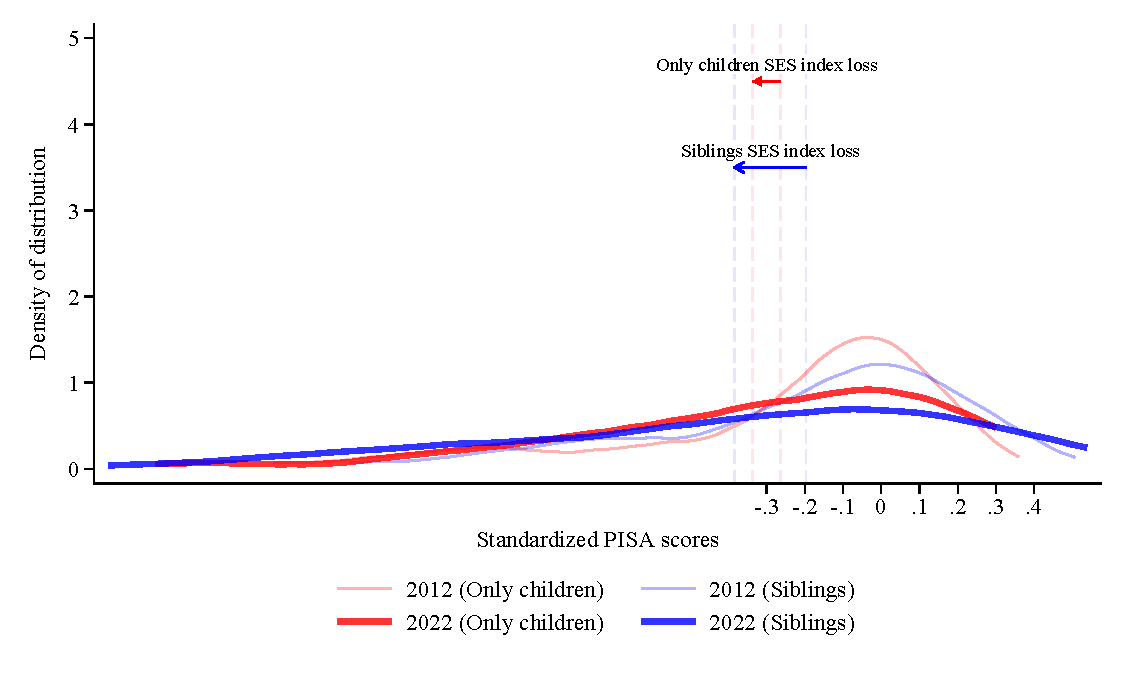
\includegraphics[width=\textwidth]{./FIGURES/Descriptive/PISA_distribution_2012_2022_ses.pdf}
        \caption{SES gaps between 2012 and 2022 for only children and children with siblings}
        \label{fig:pisa_ses}

\end{figure}

\clearpage
\subsection{Effects by age of oldest/youngest}

Results are generally noisy. Some of them can be seen in \hyperref[fig:fig_by_age_oldest]{Table \ref{fig:fig_by_age_oldest}} by age of oldest and  \hyperref[fig:fig_by_age_youngest]{Table \ref{fig:fig_by_age_youngest}} by age of youngest.


\begin{figure}[htbp]
    \centering
        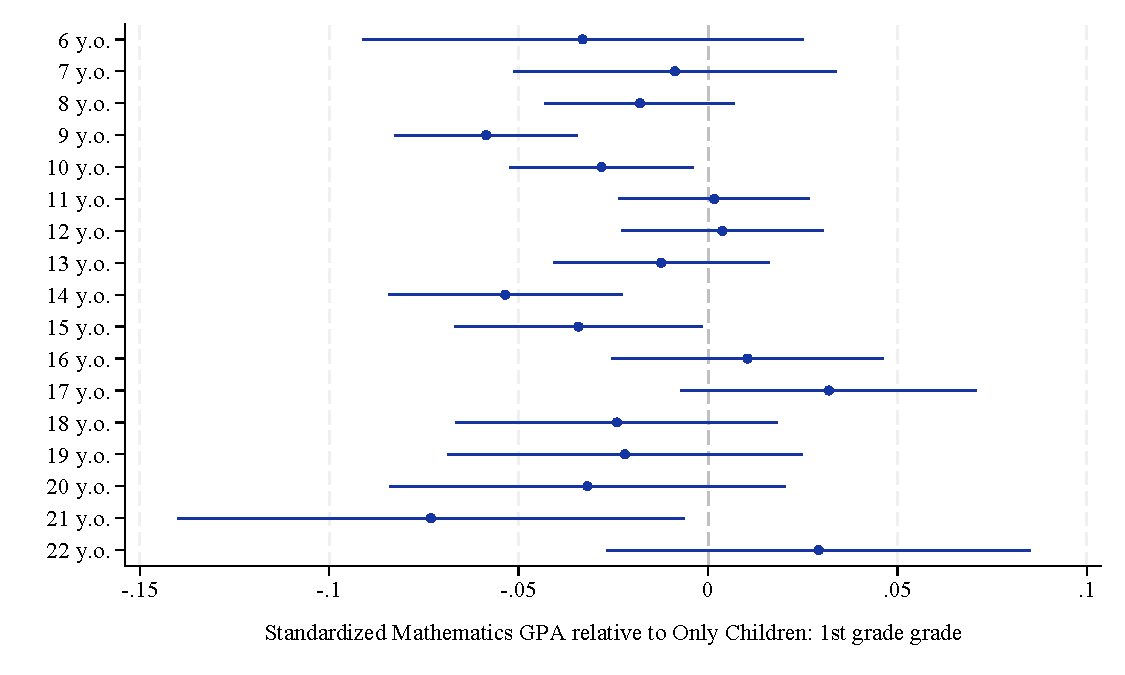
\includegraphics[width=\textwidth]{./FIGURES/TWFE/twfe_age_oldest_g1_gpa_m_adj_Tsiblings_2_Ssecond_4.pdf}
        \caption{TWFE on second-born sibling by age of oldest sibling}
        \label{fig:fig_by_age_oldest}

\end{figure}

\begin{figure}[htbp]
    \centering
    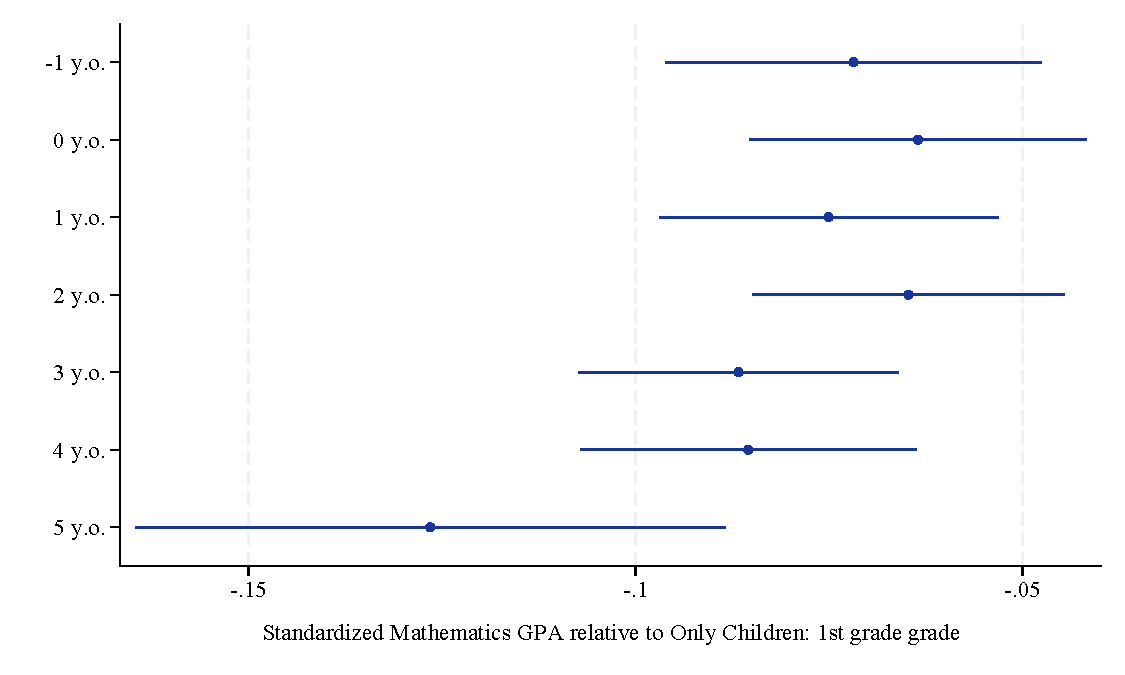
\includegraphics[width=\textwidth]{./FIGURES/TWFE/twfe_age_youngest_g1_gpa_m_adj_Tsiblings_2_Soldest_4.pdf}
        \caption{TWFE on first-born sibling by age of youngest sibling}
    \label{fig:fig_by_age_youngest}

\end{figure}

\clearpage
\subsection{Twin IV estimates}

In \hyperref[tab:twfe_twins]{Table \ref{tab:twfe_twins}} I show results of number of children on GPA using twins as an IV.

\begin{table}[h]
\centering
\caption{Effect of Family Size on GPA}
\label{tab:twfe_twins}
\resizebox{0.95\textwidth}{!}{%
\begin{tabular}{lHccccHcccc}
\hline
& \multicolumn{5}{c}{Pre-Covid} & \multicolumn{5}{c}{Covid (2020-2021)} \\
\cmidrule(lr){2-6} \cmidrule(lr){7-11}
& OLS & OLS & First & Second & N & OLS & OLS & First & Second & N \\
& (no controls) & (controls) & Stage & Stage & & (no controls) & (controls) & Stage & Stage & \\
\hline
& & & & & & & & & & \\
Instrument: first two children same sex & & & 0.050* & & 3,300,349 & & & 0.047* & & 2,809,126 \\
\quad (Sample: first and second children in families & & & (0.001) & & & & & (0.001) & & \\
\quad with two or more births) & & & & & & & & & & \\
Number of children in family & $-0.081$* & $-0.070$* & & 0.063* & & $-0.119$* & $-0.101$* & & $-0.031$ & \\
& (0.001) & (0.001) & & (0.022) & & (0.001) & (0.001) & & (0.025) & \\
Instrument: twin at second birth & & & 0.813* & & 1,589,159 & & & 0.855* & & 1,240,864 \\
\quad (Sample: First child in families with two or more & & & (0.006) & & & & & (0.006) & & \\
\quad births) & & & & & & & & & & \\
Number of children in family & $-0.090$* & $-0.056$* & & 0.012 & & $-0.125$* & $-0.085$* & & 0.009 & \\
& (0.001) & (0.001) & & (0.012) & & (0.002) & (0.002) & & (0.013) & \\
& & & & & & & & & & \\
%Instrument: twin at third birth & & & 0.819* & & 1,195,717 & & & 0.866* & & 841,770 \\
%\quad (Sample: first and second children in families & & & (0.006) & & & & & (0.006) & & \\
%\quad with three or more births) & & & & & & & & & & \\
%Number of children in family & $-0.104$* & $-0.090$* & & $-0.020$ & & $-0.118$* & $-0.101$* & & $-0.019$ & \\
%& (0.002) & (0.002) & & (0.013) & & (0.002) & (0.002) & & (0.014) & \\
%& & & & & & & & & & \\
\hline
\end{tabular}%
}
\end{table}



\newpage

